\subsection{Ca sử dụng xem danh sách địa điểm chụp}

\vspace{0.5cm}

\noindent 
\begin{tabularx}{\linewidth}{| l | X |} 
\hline 
\textbf{Mô tả} & Người dùng xem danh sách các địa điểm đã chụp từ danh sách thư viện ảnh. \\
\hline 
\textbf{Luồng cơ bản} & 1. Người dùng bấm vào nút khám phá địa điểm. \newline
                       2. Hệ thống điều hướng đến trang danh sách địa điểm đã chụp. \newline
                       3. Hệ thống lấy thông tin các địa điểm trong các bức ảnh và phân loại thành từng nhóm địa điểm chung. \newline
                       5. Hệ thống hiển thị lên giao diện. \\
\hline
\textbf{Tiền điều kiện} & - Người dùng đã đăng nhập vào hệ thống. \newline
                          - Có ít nhất 1 bức ảnh đã được cập nhật vị trí chụp ảnh. \\
\hline
\textbf{Hậu điều kiện} & - Người dùng có thể chọn địa điểm trong danh sách và xem chi tiết những ảnh chụp tại địa điểm đó. \\
\hline 
\textbf{Yêu cầu phi chức năng} & -Hệ thống lấy và nhóm dữ liệu các địa điểm không quá 2s. \\
\hline 
\end{tabularx}

\vspace{0.8cm}

\noindent 
\begin{tabular}{| c | c |}
    \hline
    \textbf{Biểu đồ hoạt động} & \textbf{Quan hệ} \\ 
    \hline
    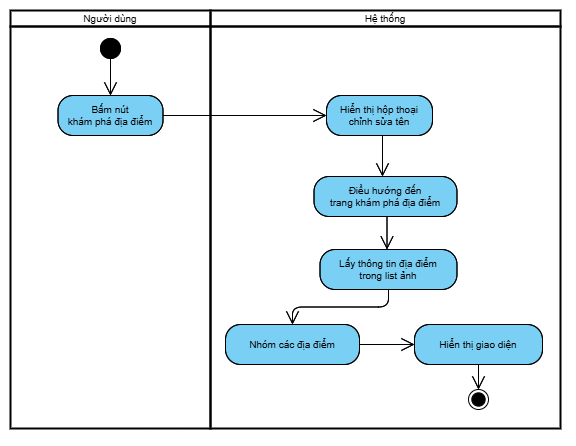
\includegraphics[width=0.6\linewidth]{figures/c3/3-3-13-activity-diagram.png} 
    &  
    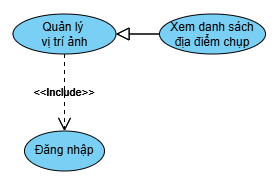
\includegraphics[width=0.35\linewidth]{figures/c3/3-3-13-relationship.png} \\ 
    \hline
\end{tabular}

\begin{figure}[H]
    \centering  
    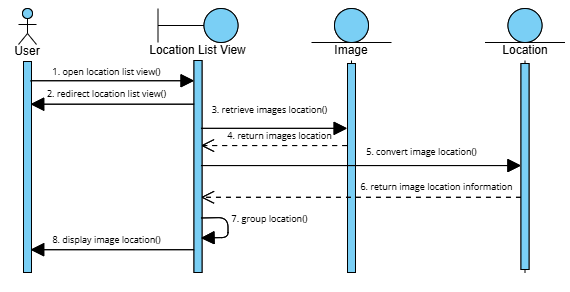
\includegraphics[width=1\textwidth]{figures/c3/3-3-13-sequence-diagram.png}
    \caption{Biểu đồ tuần tự ca sử dụng xem danh sách địa điểm chụp.}
    \label{fig:3-3-13-sequence-diagram}
\end{figure}